\Chapter{Hasonló célú alkalmazások és technológiai összehasonlításuk}

Ebben a fejezetben bemutatom a bírálati folyamat és a záróvizsga menedzselését, néhány kurzuskezelő szoftvert és az elkészítésükhöz, működtetésükhöz felhasznált technológiákat.

\Section{A bírálati folyamat és a záróvizsga menedzselése}

A bírálati folyamat és a záróvizsga menedzselése kiemelkedő fontosságú a tanulmányok vagy képzések során, mivel ezek az események segítenek az értékelésben és az eredmények összegzésében.

Általánosságban a folyamat a következő lépéseket foglalja magába:

\begin{itemize}

\item Előkészületek: A hallgatók és tanárok felkészülnek az értékelésre vagy záróvizsgára. Ez magában foglalja a tananyagok áttekintését, dokumentumok előkészítését.

\item Kritériumok meghatározása: Fontos az értékelési kritériumok vagy a záróvizsga szempontjainak meghatározása, amelyek alapján a teljesítményt értékelik. Ezek általában a tudás, készségek, alkalmazott módszerek és prezentációs készségek lehetnek.

\item Vizsgák vagy prezentációk megszervezése: Ideértve az időpontok kijelölését, helyszínek meghatározását és technikai támogatások biztosítását.

\item Értékelés: A tanárok vagy vizsgáztatók értékelik a hallgatók teljesítményét a meghatározott kritériumok alapján, legyen az írásbeli teszt, gyakorlati feladatok vagy szóbeli prezentáció.

\end{itemize}


\Section{Kurzuskezelő szoftverek}

A \textit{kurzuskezelő szoftverek} \cite{course} olyan platformok, amelyeket általában oktatási intézmények, tréningközpontok vagy vállalatok használnak a kurzusok, tanfolyamok vagy képzések hatékony kezelésére és adminisztrációjára. Ezek a szoftverek általában számos funkciót kínálnak, például regisztráció és jelentkezés kezelése, kurzusanyagok és feladatok feltöltése, tanulói teljesítmény nyomon követése, értékelési eszközök, kommunikációs eszközök és egyéb adminisztratív funkciók.

A legtöbb \textit{kurzuskezelő szoftver} online alapú, ami lehetővé teszi a hozzáférést és a kezelést bármely internetkapcsolattal rendelkező, böngészésre alkalmas eszközről. Ezek a platformok gyakran könnyen testreszabhatóak és skálázhatóak az intézmény vagy vállalat egyedi igényei szerint. Emellett sok kurzuskezelő szoftver támogatja a tanulói interakciókat és együttműködést, például csoportos munka lehetőségét vagy fórumokat biztosítva.

Ezek a szoftverek hatékony eszköztárat kínálnak az oktatási és képzési folyamatok digitalizálására és automatizálására, ami segít az adminisztratív terhek csökkentésében és a tanulási élmények javításában.

\subsection{Egységes Tanulmányi Rendszer}

A Magyarországon elterjedt felsőoktatási szoftverek egyike, az \textit{Egységes Tanulmányi Rendszer (továbbiakban: ETR)} \cite{etr}, lehetővé tette a diákok számára, hogy online platformon keresztül intézzék az oktatási intézménnyel kapcsolatos ügyeiket. Az \textit{ETR} keretében minden regisztrált hallgatónak lehetősége nyílt személyes és tanulmányi adatainak megtekintésére, pénzügyeik nyomon követésére, valamint vizsgákra jelentkezésre és kurzusok felvételére. Az \textit{ETR} technológiai alapjai az adott fejlesztőcsapat vagy az egyetem preferenciáitól függnek, így pontos fejlesztési technológiát nem lehet egyértelműen megállapítani.

2015-től kezdve az \textit{ETR} funkcionalitása fokozatosan beépült a \textit{Neptun.NET} \cite{neptun} tanulmányi rendszerbe, és az \textit{ETR}-t használó felsőoktatási intézmények 2018-ig áttértek a \textit{Neptun} rendszerére.

\subsection{Neptun}

A \textit{Neptun} \cite{neptun} egy egyetemi tanulmányi adminisztrációs alkalmazás, amely \textit{.NET} \cite{.NET} technológiával készült.  A rendszer támogatja a bírálati folyamatot és a záróvizsga menedzselését is a felsőoktatási intézményekben. A bírálati folyamat során az oktatók számos feladatot végeznek, például tanulmányi eredmények értékelése, visszajelzések megadása, valamint a hallgatók előrehaladásának nyomon követése. A rendszer lehetőséget biztosít az oktatóknak arra, hogy ezeket a feladatokat hatékonyan elvégezzék, beleértve az eredmények rögzítését és a visszajelzések megadását is.

A záróvizsga menedzselése is fontos része a \textit{Neptun} platformnak. Ennek során az intézményeknek lehetőségük van előre meghatározott időpontokban és helyszíneken szervezni a záróvizsgákat, valamint regisztrálni a hallgatókat ezekre a vizsgákra.

A \textit{Neptun} szolgáltatás általában rugalmas konfigurációs lehetőségeket kínál az intézmények számára, hogy testreszabhassák a bírálati folyamatot és a záróvizsga menedzselését (\ref{fig:neptunzv} ábra) az adott intézet saját igényeihez és eljárásaihoz. Ezáltal az intézmények hatékonyan tudják kezelni ezeket a fontos tanulmányi folyamatokat, és biztosítani tudják a hallgatók és oktatók számára az átlátható kommunikációt és adminisztrációt.

\begin{figure}[h]
\centering
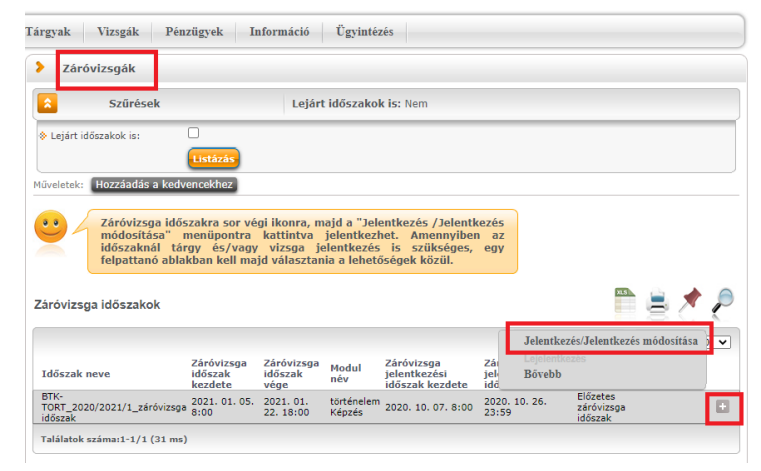
\includegraphics[scale=0.7]{images/Neptun.png}
\caption{Záróvizsga jelentkezés a \textit{Neptun} rendszerben \cite{neptunzv}}
\label{fig:neptunzv}
\end{figure}

\newpage
\subsection{KRÉTA}

A \textit{KRÉTA (Köznevelési Regisztrációs és Tanulmányi Alaprendszer)} \cite{kreta} kurzuskezelő szoftver számos funkciót kínál a tanulmányi folyamatok hatékony kezelésére és adminisztrációjára, ami PHP \cite{PHP} technológiával készült. Az oktatók számára lehetőség van a tanulmányi eredmények értékelésére (\ref{fig:kreta} ábra), visszajelzések megadására, valamint a diákok teljesítményének nyomon követésére. Ezáltal az oktatók hatékonyan tudják értékelni a diákok munkáját és fejlődését, és szükség esetén visszajelzést adni nekik a további fejlődés érdekében.

A bírálati folyamatok integrációja a \textit{KRÉTA} kurzuskezelő rendszerébe lehetővé teszi az intézmények számára, hogy átláthatóan és hatékonyan kezeljék az értékelési folyamatokat. Emellett segíti az oktatókat abban is, hogy időben és pontosan értékeljék a diákok munkáját, és visszajelzést adhassanak a tanulmányi előrehaladásukról. Így a \textit{KRÉTA} nemcsak a tanulmányi folyamatok kezelését segíti, hanem a bírálati folyamatokat is integrálja, hogy teljeskörű támogatást nyújtson az oktatási intézmények számára.
\begin{figure}[h]
\centering
\includegraphics[scale=0.4]{images/Kréta.png}
\caption{Értékelés a \textit{KRÉTA} rendszerben \cite{kreta_jegy}}
\label{fig:kreta}
\end{figure}
\newpage
\subsection{Blackboard Learn}

A \textit{Blackboard Learn} \cite{blackboard_learn} egy kifinomult e-learning platform, melyet széles körben használnak oktatási intézmények világszerte. Ez az alkalmazás lehetővé teszi az oktatók számára, hogy létrehozzanak és kezeljenek online tananyagokat, interaktív kurzusokat, valamint feladatokat és teszteket. A hallgatók számára a \textit{Blackboard Learn} egy hozzáférhető, felhasználóbarát felületet biztosít, ahol könnyen hozzáférhetnek a tananyagokhoz, kommunikálhatnak az oktatókkal és társaikkal, valamint beadhatják feladataikat és vizsgáikat.

\overfullrule=0pt Az oktatók az alkalmazáson keresztül képesek értékelni a hallgatók munkáját, visszajelzéseket adni nekik, valamint nyomonkövetni az előrehaladásukat és teljesítményüket. Emellett a \textit{Blackboard Learn} lehetőséget biztosít az intézményeknek a vizsgák szervezésére, menedzselésére és értékelésére (\ref{fig:blackboard_learn_review} ábra). Ez az alkalmazás segít az oktatási folyamatok digitalizálásában és hatékonyabbá tételében, elősegítve a hallgatók és oktatók közötti interakciót és együttműködést.

\begin{figure}[h]
\centering
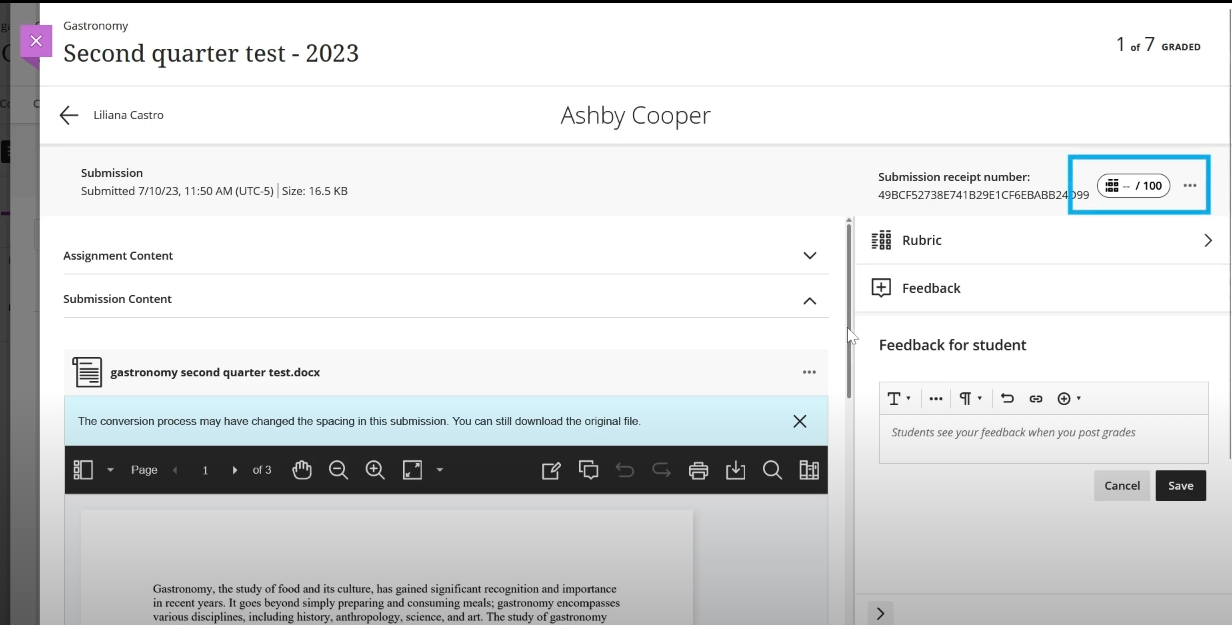
\includegraphics[scale=0.4]{images/Blackboard_Learn.png}
\caption{Értékelés és bírálat készítése a \textit{Blackboard Learn} rendszerben  \cite{blackboard_learn_review}}
\label{fig:blackboard_learn_review}
\end{figure}

\subsection{Moodle}

A \textit{Moodle} \cite{moodle} egy nyílt forráskódú e-learning platform, amelyet a tanulás és oktatás támogatására terveztek. Rugalmas és testreszabható jellege révén széles körű oktatási környezetekben használják, legyen az iskolai, egyetemi vagy vállalati. A \textit{Moodle} lehetővé teszi az oktatóknak, hogy létrehozzanak online kurzusokat, kezeljék a tananyagokat, kommunikáljanak a diákokkal és értékeljenek. A Miskolci Egyetem által használt e-learning rendszer is ezen alapul, így a hallgatók és oktatók számára ismerős környezetet biztosít.
\\
A platform rendelkezik számos funkcióval, többek között:

\begin{enumerate}


\item Kurzuskezelés: A \textit{Moodle} segítségével könnyedén létrehozhatók és kezelhetők online kurzusok (\ref{fig:moodle} ábra). Lehetőség van multimédiás tartalmak, tesztek, házi feladatok és egyéb oktatási anyagok feltöltésére és megosztására.

\item Kommunikáció és együttműködés: A tanárok és diákok könnyen kommunikálhatnak egymással a fórumok, üzenetküldés és csoportmunka funkciók segítségével. Ez lehetővé teszi az interaktív tanulást és az együttműködést az online térben.

\item Értékelés és visszajelzés: A \textit{Moodle} lehetővé teszi a tanárok számára, hogy értékeljék a diákok teljesítményét online tesztek, feladatok és vizsgák segítségével. A diákok pedig azonnali visszajelzést kapnak a munkájukról, ami segíti a tanulási folyamatot.

\item Testreszabhatóság és bővíthetőség: A \textit{Moodle} nyílt forráskódú platform, így lehetőség van arra, hogy a felhasználók testre szabhassák az igényeiknek megfelelően.

\end{enumerate}


\begin{figure}[h]
\centering
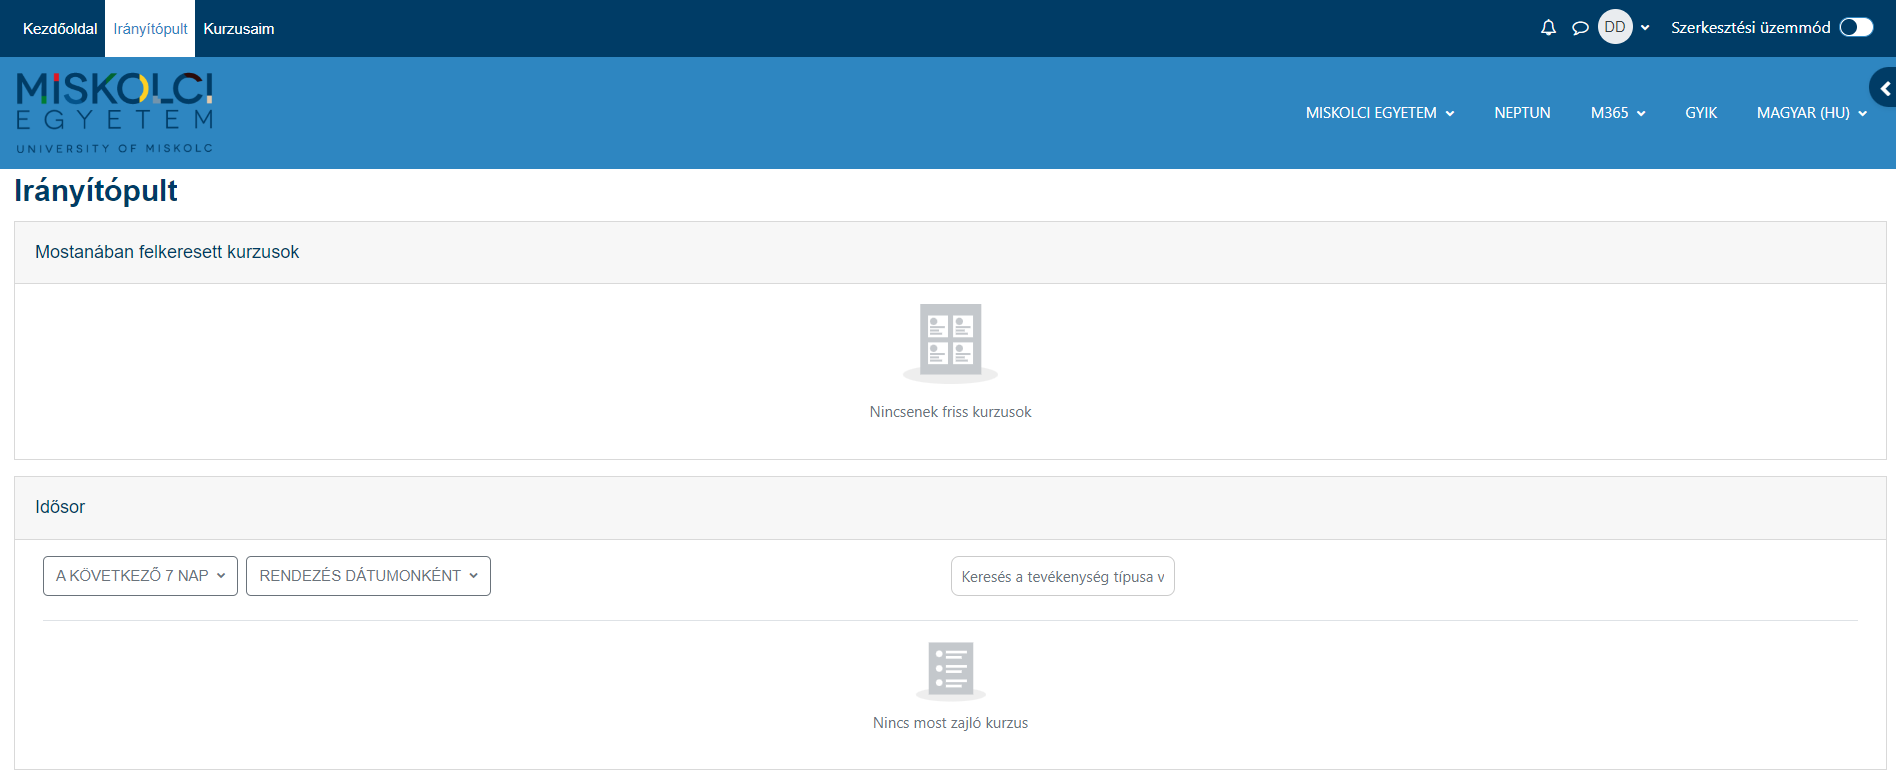
\includegraphics[width=\textwidth]{images/moodle.png}
\caption{A Miskolci Egyetem \textit{Moodle} rendszer kezelőfelülete \cite{moodle miskolci}}
\label{fig:moodle}
\end{figure}


\Section{Felhasznált technológiák}

A felhasznált technológiák megválasztásakor elterjedt és stabil eszközök alkalmazása volt a cél, mivel ezek a megbízható platformok lehetővé teszik a hatékony munkavégzést és minimalizálják az esetleges technikai problémák kockázatát.


\subsection{Adatbázis}

Ahhoz, hogy hatékonyan kezeljem az adatokat a \textit{MySQL} \cite{MySQL} relációs adatbázis-kezelő rendszert választottam. A \textit{MySQL} rendszer biztosítja a szükséges funkcionalitást az adatbázis létrehozásához és kezeléséhez, valamint lehetővé teszi az adatok gyors és hatékony lekérdezését.

Az adatbázis-kezeléshez a \textit{MySQL Community Edition} \cite{MySQL Community Edition} csomag részeként könnyen elérhető \textit{MySQL Workbench} \cite{MySQL_Workbench} alkalmazást választottam. Ennek segítségével könnyedén létrehozhatom az adatbázis sémáját, végrehajthatom az \textit{SQL} \cite{SQL} utasításokat és optimalizálhatom azokat. A \textit{MySQL Workbench} számos hasznos eszközt kínál, mint például a szintaxiskiemelést és az automatikus kiegészítést, ami jelentősen megkönnyíti a fejlesztési folyamatot.

A \textit{MySQL} helyett választható lett volna például az \textit{SQLite}, \textit{MariaDB}. Emellett az adatok nyilvántartására maximálisan alkalmas a \textit{MongoDB} dokumentumorientált adatbázismotor is, mivel a kezelendő információk nem teszik elengedhetetlenné relációs adatbázis választását.


\subsection{Java Spring Boot}

A webalkalmazásom backend részéhez a \textit{Java} \cite{java} programozási nyelvet választottam. A \textit{Java} egy kiválóan használható, objektumorientált nyelv, amely széles körben elterjedt a fejlesztői közösségben.

A backend implementációjához a \textit{Spring Boot} \cite{spring_boot} keretrendszert választottam, amely segíti a gyors és egyszerű webalkalmazások fejlesztését. A \textit{Spring Boot} automatikus konfigurációval rendelkezik, ami megkönnyíti a fejlesztési folyamatot. Támogatja az \textit{MVC (Model-View-Controller)} \cite{mvc} programtervezési mintát, és beágyazott \textit{Tomcat} \cite{Tomcat} szerveren futtatja az alkalmazást.\\ 
\\
Az \textit{MVC} modell (\ref{fig:mvc} ábra) három fő logikai egységből áll melyek a következők:

\begin{itemize}
\item \textbf{Controller:} Az \textit{MVC (Model-View-Controller)} modellben a vezérlő feladata a felhasználói interakciók kezelése és az üzleti logika irányítása. A vezérlő fogadja a kéréseket a felhasználótól, feldolgozza azokat, majd frissíti a modellt vagy változtatást eszközöl a nézeten.
\item \textbf{View:} A nézet az adatok megjelenítéséért felelős rész. A modellből származó adatokat a felhasználó számára értelmezhető formában jeleníti meg. A nézetek lehetnek grafikus felületek, weboldalak, vagy akár más típusú kimenetek is.
\item \textbf{Model:} A modell reprezentálja az alkalmazás adatait és üzleti logikáját. Az adatokat tárolja, feldolgozza és manipulálja a modell, valamint a szükséges műveleteket elvégzi az adatok tartós tárolásához vagy az alkalmazás állapotának fenntartásához. A modell nem kommunikál közvetlenül a felhasználóval, helyette a vezérlő által történik az adatok elérése és kezelése.
\end{itemize}

\begin{figure}[h]
\centering
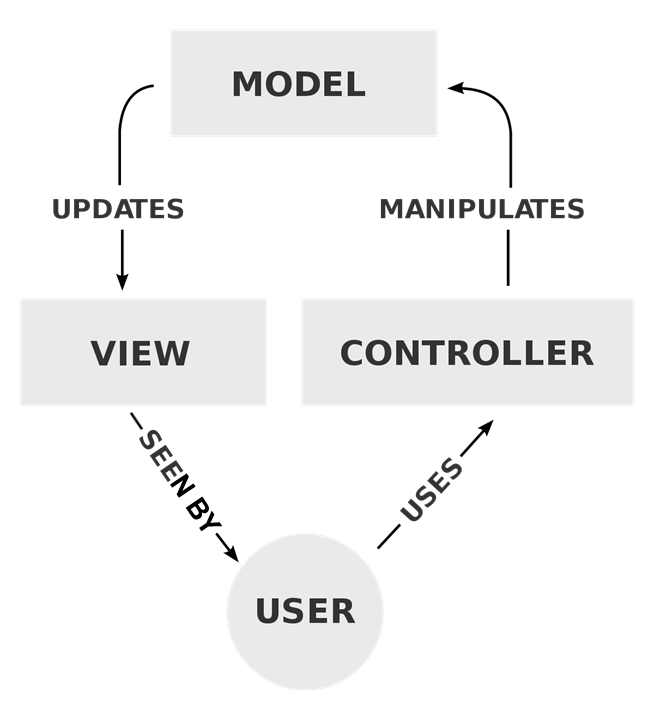
\includegraphics[scale=0.50]{images/MVC_modified.png}
\caption{\textit{MVC} modell \cite{mvc}}
\label{fig:mvc}
\end{figure}

Bár más technológiák is elérhetőek lettek volna, mint például a \textit{Node.js}, a \textit{Python} \textit{Django} vagy a \textit{C\# ASP.NET Core},  azonban tapasztalataim alapján a \textit{Java} \cite{java} és kifejezetten a \textit{Spring Boot} \cite{spring_boot} a legmegfelelőbb választásnak tűnt a projekt szempontjából.

\subsection{Angular}

A fejlesztett webalkalmazás vékony kliens alapú, ami azt jelenti, hogy a szükséges funkciók és üzleti logika a távoli szerveroldalon, vagyis a backenden kerülnek implementálásra. A kommunikáció a kliens és a szerver között \textit{HTTP} \cite{http} protokollon keresztül zajlik, ami egy alkalmazás szintű, állapotmentes kérés-válasz alapú protokoll elosztott rendszerek számára. A \textit{GET, POST, PUT és DELETE} \textit{HTTP} metódusokat használom az adatok kezelésére.

Az alkalmazás frontend részét az \textit{Angular} \cite{angular} keretrendszer segítségével valósítottam meg. Az \textit{Angular} egy nagy teljesítményű, bővíthető és funkciókban gazdag frontend eszközkészlet, amely lehetővé teszi összetettebb webalkalmazások fejlesztését különböző komponensekből, amelyek \textit{HTML} \cite{html}, \textit{TypeScript} \cite{ts} és \textit{CSS} \cite{css} fájlokra épülnek. A felhasználói felület megjelenésének stílusához \textit{Bootstrap} \cite{bootstrap} eszközkészletet is alkalmaztam, ami rengeteg \textit{HTML} és \textit{CSS} alapú tervezősablont és mintát tartalmaz számos komponenshez.

Lehetőség lett volna a \textit{Vue} \cite{vue} vagy a \textit{React} \cite{react} használatára is a webalkalmazás frontendjének megvalósításához, de az \textit{Angular} \cite{angular} mellett döntöttem. Az \textit{Angular} széles körű támogatottsága és népszerűsége miatt könnyebb volt találni hozzá dokumentációt, oktatóanyagokat és közösségi támogatást, ami gyorsabb fejlesztést eredményezett.
